\documentclass[journal]{IEEEtran}
\usepackage[a5paper, margin=10mm]{geometry}
\usepackage{tfrupee} % Include tfrupee package
\usepackage{gvv-book}
\usepackage{gvv}
\usepackage{pdfpages}
\usepackage{fbox} % For extended fbox features

\setlength{\intextsep}{10pt} % Space between text and floats

\setlength{\headheight}{1cm} % Set the height of the header box
\setlength{\headsep}{0mm}     % Set the distance between the header box and the top of the text

\makeindex
\begin{document}
	
	\bibliographystyle{IEEEtran}
	\onecolumn
	
	\title{
		CLOCK WITH KMAPS
		
		\large{EE1003 : Scientific Programming for Electrical Engineers}
		
		Indian Institute of Technology Hyderabad
	}
	
	\author{Yellanki Siddhanth (EE24BTECH11059)}
	
	\maketitle
	
	\renewcommand{\thefigure}{\theenumi}
	\renewcommand{\thetable}{\theenumi}
	
	\section{Introduction}
	The digital clock system described here utilizes Karnaugh maps (K-Maps) for incrementing time units and a multiplexing technique to display time on six seven-segment displays using only a single BCD. This report outlines the system's architecture, operation, and implementation details.
	
	\section{Circuit Description}
	The circuit consists of the following key components:
	\begin{enumerate}
		\item Arduino Atmel328p Microcontroller
		\item Six Seven-Segment Displays
		\item IC7447 BCD for the Seven-Segment Displays
		\item Wires
		\item 220$\Omega$ Resistors for the Seven-Segment Displays
	\end{enumerate}
			\includepdfset{pages=-} % Include all pages from the PDF
	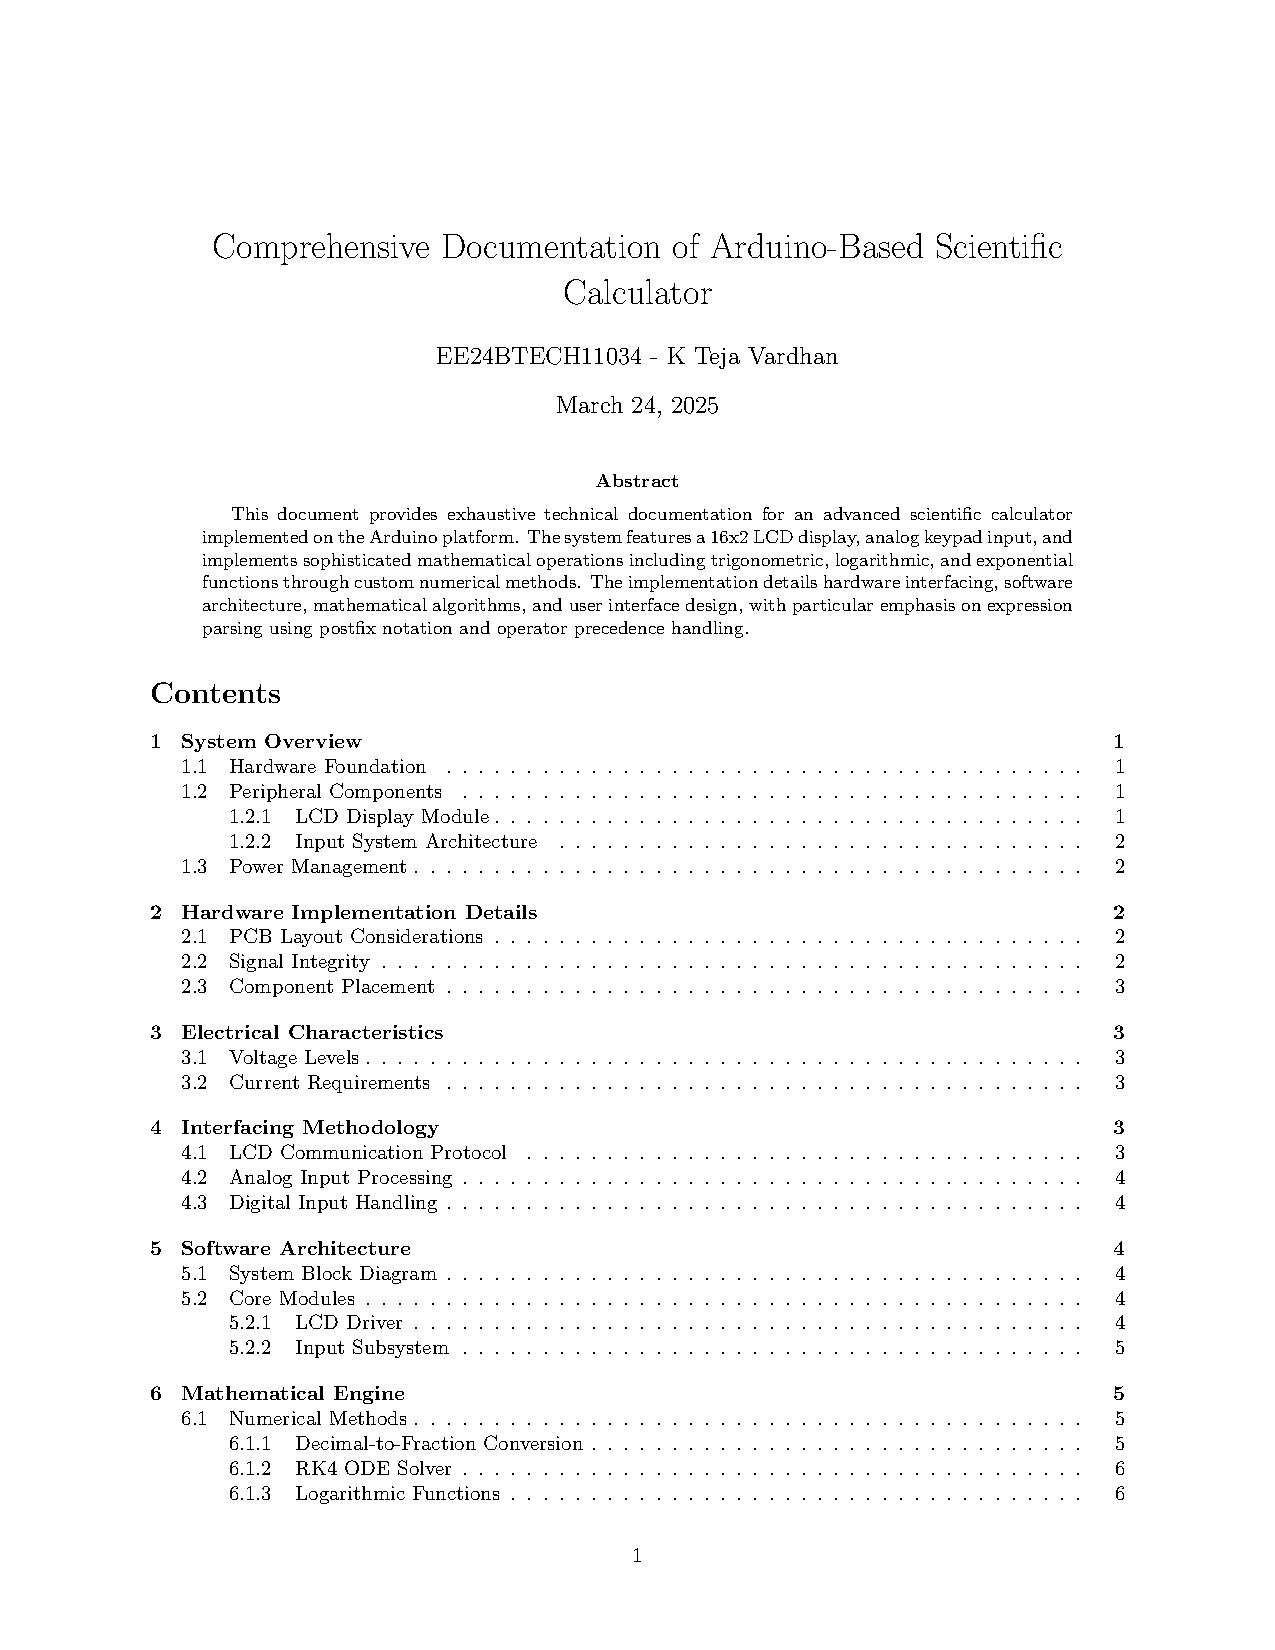
\includepdf{figs/clock.pdf} % Include the first PDF
	
	\begin{figure}[h!]
	    \centering
	    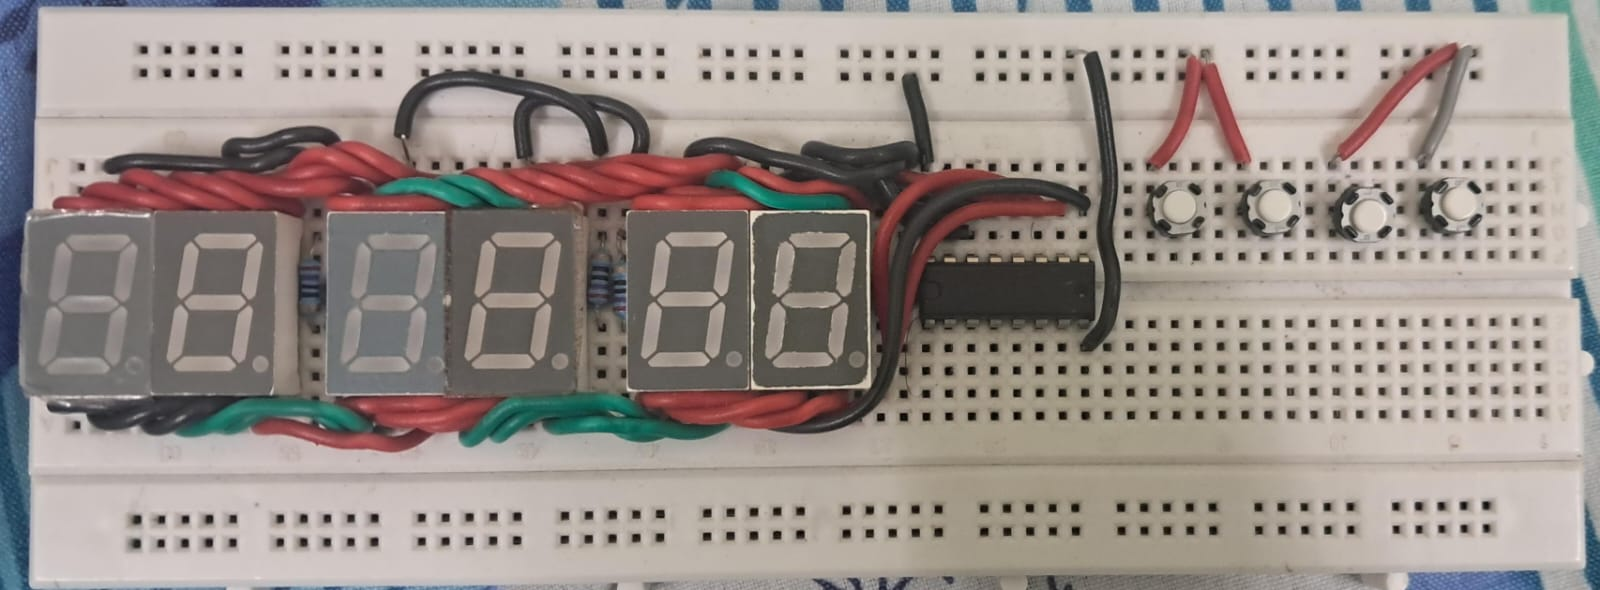
\includegraphics[width=0.8\textwidth]{figs/circuit.jpeg}
	    \caption{Circuit Diagram}
	\end{figure}
	
	\section{Multiplexing Technique}
	Multiplexing is achieved by connecting all inputs of the seven-segment displays to a single BCD. Digital pins are connected to the common of each display, allowing selective display of the BCD output. The displays are alternated with a 2$\mu$s time gap, creating the illusion of simultaneous operation.
	
	\section{K-Map Incrementing Logic}
	The incrementing logic for each display is implemented using decade counters. For the unit's place of the seconds, the logic is as follows:
	\begin{align}
		A_1 &= \overline{W_1}; \\
		B_1 &= (W_1 \land \overline{X_1} \land \overline{Z_1}) \lor (\overline{W_1} \land X_1);\\
		C_1 &= (\overline{X_1} \land Y_1) \lor (\overline{W_1} \land Y_1) \lor (W_1 \land X_1 \land \overline{Y_1});\\
		D_1 &= (\overline{W_1} \land Z_1) \lor (W_1 \land X_1 \land Y_1).
	\end{align}
	For the ten's place of the seconds, which varies from 0 to 5:
	\begin{align}
		A_2 &= \overline{W_2};\\
		B_2 &= (\overline{Y_2} \land \overline{X_2} \land W_2) \lor (\overline{W_2} \land X_2);\\
		C_2 &= (\overline{W_2} \land Y_2) \lor (X_2 \land W_2);\\
		D_2 &= 0.
	\end{align}
	To synchronize the ten's place increment with the unit's place reaching 9, an additional variable $C$ is used:
	\begin{align}
		C &= W_1 \land \overline{X_1} \land \overline{Y_1} \land Z_1 \\
		A_2 &= (A_2 \land C) \lor (W_2 \land \overline{C}) \\
		B_2 &= (B_2 \land C) \lor (X_2 \land \overline{C}) \\
		C_2 &= (C_2 \land C) \lor (Y_2 \land \overline{C}) \\
		D_2 &= (D_2 \land C) \lor (Z_2 \land \overline{C}).
	\end{align}
	Now, using the above logic, the ten's digit of seconds only updates when the unit's digit previously is 9. This logic can be reapplied for the next display, i.e., the unit's digit of the minutes:
	\begin{align}
		A_3 &= \overline{W_3}; \\
		B_3 &= (W_3 \land \overline{X_3} \land \overline{Z_3}) \lor (\overline{W_3} \land X_3);\\
		C_3 &= (\overline{X_3} \land Y_3) \lor (\overline{W_3} \land Y_3) \lor (W_3 \land X_3 \land \overline{Y_3});\\
		D_3 &= (\overline{W_3} \land Z_3) \lor (W_3 \land X_3 \land Y_3).
	\end{align}
	The value of $C$ for this case is:
	\begin{align}
		C &= W_2 \land \overline{X_2} \land Y_2 \land \overline{Z_2} \land W_1 \land \overline{X_1} \land \overline{Y_1} \land Z_1.
	\end{align}
	
	\section{Control Implementation}
	Four buttons connected to PORTD control the clock:
	\begin{enumerate}
		\item Pressing the first button will pause/play the clock.
		\item Pressing the second button while paused will increment the seconds.
		\item Pressing the third button while paused will increment the minutes.
		\item Pressing the fourth button while paused will increment the hours.
	\end{enumerate}
	To increment the minutes, the incrementing logic is run 60 times. Similarly, incrementing hours requires running the loop 3600 times.
	
	\section{Software Implementation}
	EEPROM persistence is implemented for all variables ($W_i, X_i, Y_i, Z_i, A_i, B_i, C_i, D_i$), ensuring the clock retains its time when powered off.
	
	\section{Conclusion}
	This digital clock system effectively utilizes Karnaugh maps and multiplexing to display time on multiple seven-segment displays. The system's design and implementation provide a practical example of integrating logical incrementing techniques with efficient display methods.

	\section*{Code Requirements}
	The code is located in the following directory:\\  \fbox{%
		\parbox{\textwidth}{
			/codes/final/code.c
		}%
	} It can be compiled and uploaded directly using the Makefile.
	
\end{document}
